\documentclass[mres, copyrightpage, examinerscopy]{mqthesis}
\usepackage{natbib}
\usepackage[scientific-notation=true]{siunitx}
%----------------------------------------------------------
% OPTIONS
% Options you can use in the documentclass above:
%
% phd/mres/hons = set the degree text [default=phd if absent]
% copyrightpage = print a copyright page on the back 
%                 of the title page [default=false]
% examinerscopy = print "Examiner's Copy" of title page and 
%                 change linespacing to 1.5 [default=false]
% greychapternumbers = print large chapter numbers in grey
%                 instead of MQ corporate "sand"
%---------------------------------------------------------- 

% this shows what labels you are using for cross references
% \usepackage{showkeys} 

%---------------------------------------------------------- 
% STRUCTURE
% this document is a skeleton which pulls in the meat of the thesis
% from other files. Comment out and add lines as appropriate.
%---------------------------------------------------------- 

% N.B. for final printing you may want to remove the 'examinerscopy' 
% option, which will remove 'Examiner's Copy' from title page
% and change the linespacing to single space for a professional look
% ... just saying. Check figure placement though!

\begin{document}

%---------------------------------------------------------- 
% FRONT
% Acknowledgements, titlepage, abstract, list of publications
%---------------------------------------------------------- 
\frontmatter

\title{Insert thesis title here}
\author{Praveen Nisal Jayasuriya Daluwathumullagamage}
\department{Physics}  % put your department here

\titlepage

\chapter{Acknowledgements}

I would like to thank my wife Gazala who supported me and pushed me to do more astronomy and apply to the Master's program at Macquarie University. I would also like to thank my family in Sri Lanka who support everything I do and encouraged me to follow my interests no matter what. I would not be completing this work if not for my family.

A big thank you to my supervisor Dr Daniel Zucker who in addition to providing valuable feedback, guided and believed in me every step of the way. Your friendship and mentorship has made this journey so much more enjoyable. Thank you to Dr Ben Montet at UNSW who introduced me to the astronomy community in Australia and encouraged me to apply to Macquarie University. As an immigrant and someone who had no formal training in astronomy until this point, I owe a debt of gratitude.

Many thanks to Dr Sarah Martell at UNSW for the early feedback and guidance on P Cygni spectra. Thank you to Dr Gregor Traven at Lund University for his valuable feedback and sanity checks towards the end of the project. Thanks to Arv Hughes, Dr Sven Buder and Dr Klemen Čotar and the various members of the GALAH science team and HDR cohort at Macquarie University who provided feedback and support during various forums and meetings throughout the last year - your kindness, generosity and camaraderie is highly appreciated. Finally, many thanks to all my friends, particularly Nuzhi Meyen in Sri Lanka for his input on the mathematics of machine learning and my many friends in Sydney who have had to endure me talking about astronomy 24/7/365.
\chapter{List of Publications}

\begin{itemize}
\item[$\bullet$] insert author list \emph{insert paper title}.  (submitted to
	insert journal name)
\item[$\bullet$] insert author list \emph{insert paper title}.  
        insert journal name \textbf{insert volume number}, 
        insert article or page number (insert year)
\end{itemize}

\chapter{Abstract}

This is my abstract.  This is what I've spent the last $x$ years working on,
and I'm going to tell you about now.


\tableofcontents
% comment out these as required for your discipline
\listoffigures
\listoftables

%---------------------------------------------------------- 
% MAIN
% include chapters as neededlmodern
%---------------------------------------------------------- 
\mainmatter

% Introduction
\chapter{Introduction}
\section{The Data Deluge in Modern Spectroscopic Surveys}
Modern large scale spectroscopic surveys generate hundreds of thousands or even millions of spectra. The analysis of these high volume data-sets presents a significant challenge to the researcher as well as to compute infrastructure and engineering. Additionally, if the data is collected by a high resolution instrument, the researcher will face the challenge of wrangling and analysing individual data points with dimensions at the scale of several thousands per spectrum \cite{buder2021galah+}. 
When the number of data points are of the order of hundreds of thousands (or millions) and when each data point has a dimensionality of several thousands, it becomes impractical and perhaps even infeasible to process and analyse this data using manual methods such as naked eye observations of spectral plots. Unless the science goals have been set to bias a survey specifically towards star forming regions (for example) \cite{traven2015gaia}, these surveys will contain a significant majority of spectra that are presumably typical. Thus the identification and classification of atypical objects such as emission-line stars for example, presents a serious challenge in addition to those mentioned previously.

\begin{table}[]
\begin{center}
\begin{tabular}{|c|c|c|}
\hline
\textbf{Survey} & \textbf{Number of Spectra} & \textbf{Resolution} \\ \hline
Gaia ESO        & $\sim$150,000              & High                \\ \hline
LAMOST          & $\sim$10,000,000           & Low                 \\ \hline
APOGEE          & $\sim$250,000              & High                \\ \hline
RAVE            & $\sim$600,000              & High                \\ \hline
GAIA            & $\sim$100,000,000          & Low                 \\ \hline
\end{tabular}
\caption{Modern spectroscopic surveys generate high volume, and often high resolution data.}
\label{table:draglift1}
\end{center}
\end{table}

These surveys use data analysis pipelines to generate stellar parameters and often use template spectra that are typical. It has been demonstrated that the use of these so called non-peculiar baselines can impact the accurate determination of effective temperature \cite{cayrel2011halpha}\cite{amarsi2018effective}\cite{giribaldi2019accurate} as well as stellar mass \cite{ness2016spectroscopic}\cite{bergemann2016gaia}. In addition to providing significant insight into stellar evolutionary pathways, the identification of atypical emission-line stars can thus improve the accurate determination of stellar parameters. To achieve this outcome, once identified and classified, these spectra can be removed from the primary data analysis pipeline containing typical spectra and can be reduced by secondary pipelines more suited for their peculiarities. 
The detection of atypical signals or data points in significantly larger more typical populations of data presents itself well to modern machine learning techniques. To-date, a variety of machine-learning techniques have been applied to the identification of emission-line stars and in particular H$\alpha$ emission-line stars . However, major drawbacks and challenges remain both in the identification and classification of emission-line stars despite the use of popular and seemingly robust machine learning techniques such as dimensionality reduction, k-means clustering and neural networks. Given these drawbacks, it is not uncommon that manual methods are still being used for identification and classification of emission-line stars \cite{zhang2021catalog}. A more detailed review of these efforts are presented in Chapter 3. 



\section{P Cygni Stars}
P Cygni (or 34 Cygni) is a luminous blue variable star (LBV) that has been studied extensively \cite{1953PDAO....9....1B, hutchings1969expanding, elliott20225, underhill1966supergiants,mizumoto2018newly}. Willem Janszoon Blaeu, a Dutch cartographer and student of the astronomer Tycho Brahe is considered to have provided the first known set of observations of 34 Cygni in the year 1600 \cite{deGrootPCygni}. The stellar spectrum of 34 Cygni is peculiar. It exhibits the characteristics of a B type supergiant except that almost all absorption lines are blue shifted with a red shifted emission component \cite{hutchings1969expanding}. This characteristic line profile can be clearly observed in proximity to the H$\alpha$ line which is placed at \textasciitilde 6563\r{A} \cite{zhang2021catalog,traven2015gaia}

P Cygni type stars or simply, \emph{P Cygni stars} are stars that exhibit line profiles that are similar to the characteristic profile of 34 Cygni. The spectra of these stars show characteristic absorption, emission and wide absorption sub-components \cite{zhang2021catalog}. The red shifted absorption (or blue shifted emission) counterpart to P Cygni stars have also been observed. These now belong to a class of objects known as the Inverted P Cygni stars or \emph{Inverse P Cygni stars}. 

\begin{figure}[t]
\centering
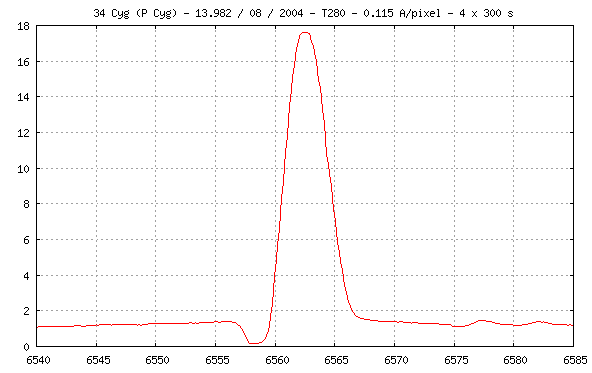
\includegraphics[scale=.40]{figures/34cygni.png}
\caption{The normalised spectrum of 34 Cygni around H$\alpha$.}
\end{figure}

It is hypothesised that distinct physical processes within these stars generate the respective line profiles \cite{hou2016catalog}. Beals was the first to demonstrate that P Cygni and Inverse P Cygni line profiles can be explained by the interaction between the stellar disk of a hot, massive young star and the expanding or contracting shell of gas surrounding the star \cite{1953PDAO....9....1B}. 

\begin{figure}[h]
\centering
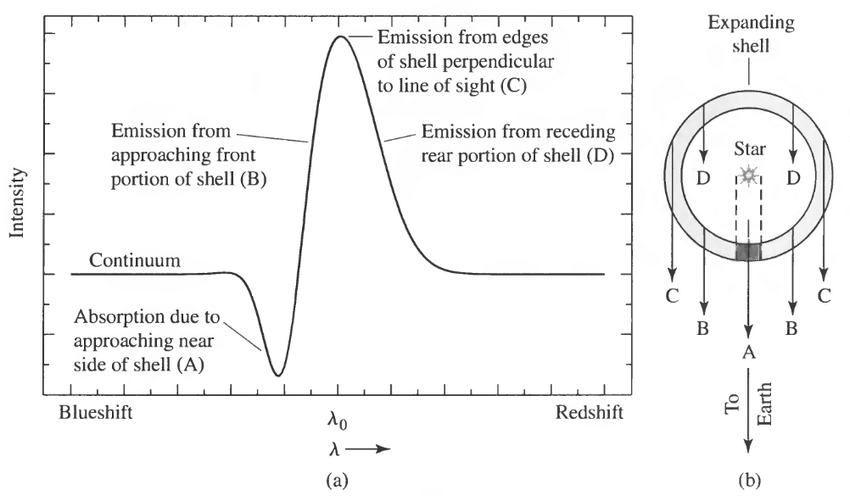
\includegraphics[scale=.40]{figures/expandingpcygni.png}
\caption{Cartoon depicting the physical mechanism by which a P Cygni line profile is generated. Reproduced from Kasai (2013)\cite{kasai2013type}.}
\end{figure}

The P Cygni line profile observed is thus a result of an expanding shell of gas around the main disk of the young hot star. The segment of this shell along the ling of sight contributes to the generation of the absorption line in the spectrum. An average or normal main sequence star will only show a significantly deep absorption line/trough near H$\alpha$. However, note that in the case of P Cygni, the regions B, C and D of the shell contribute to an emission line. This emission line can occur near H$\alpha$. As we move from B to C, the intensity of the emission line increases until we reach the edge of the shell. Beyond this point the shell is receding with respect to the line of sight and the intensity of the emission line decreases. It is believed that the opposite process occurs in the case of an inverse P Cygni star. In this case, the shell of gas is contracting and this inflow is responsible for the blue shifted emission line, often to the left of H$\alpha$.

\begin{figure}[h]
\centering
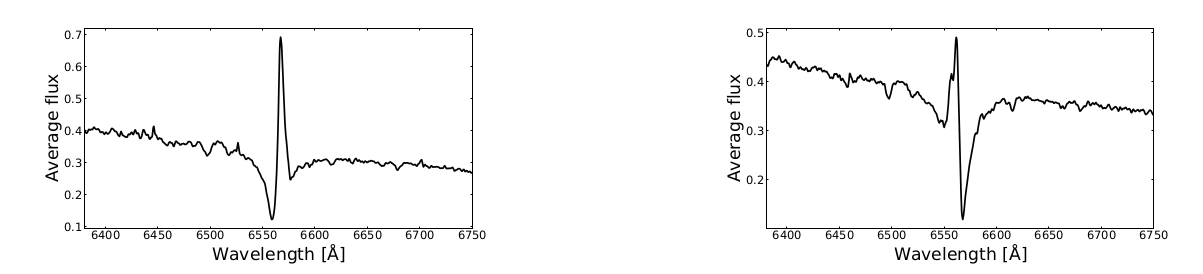
\includegraphics[scale=.50]{figures/p cygni and inverse p cygni.png}
\caption{A P Cygni spectrum (left) and an inverse P Cygni spectrum (right) from LAMOST Data Release 7. Reproduced from Zhang (2021)\cite{zhang2021catalog}.}
\end{figure}

\section{Morphological Classification}
One of the first modern attempts at identifying and characterising P Cygni stars was by Beals (1953) \cite{1953PDAO....9....1B}. This work compiled Northern Hemisphere observations of P Cygni stars into a comprehensive catalog. This catalog was compiled by examining spectra using the naked eye, during a period of observation between the years 1928 and 1946. The catalog was then used to generate hypotheses of how P Cygni stars may exchange material with their surroundings via accretions, inflows and outflows. The morphological properties of the spectra were then used to calculate the wind velocities of inflows and outflows. 

\begin{figure}[t]
\centering
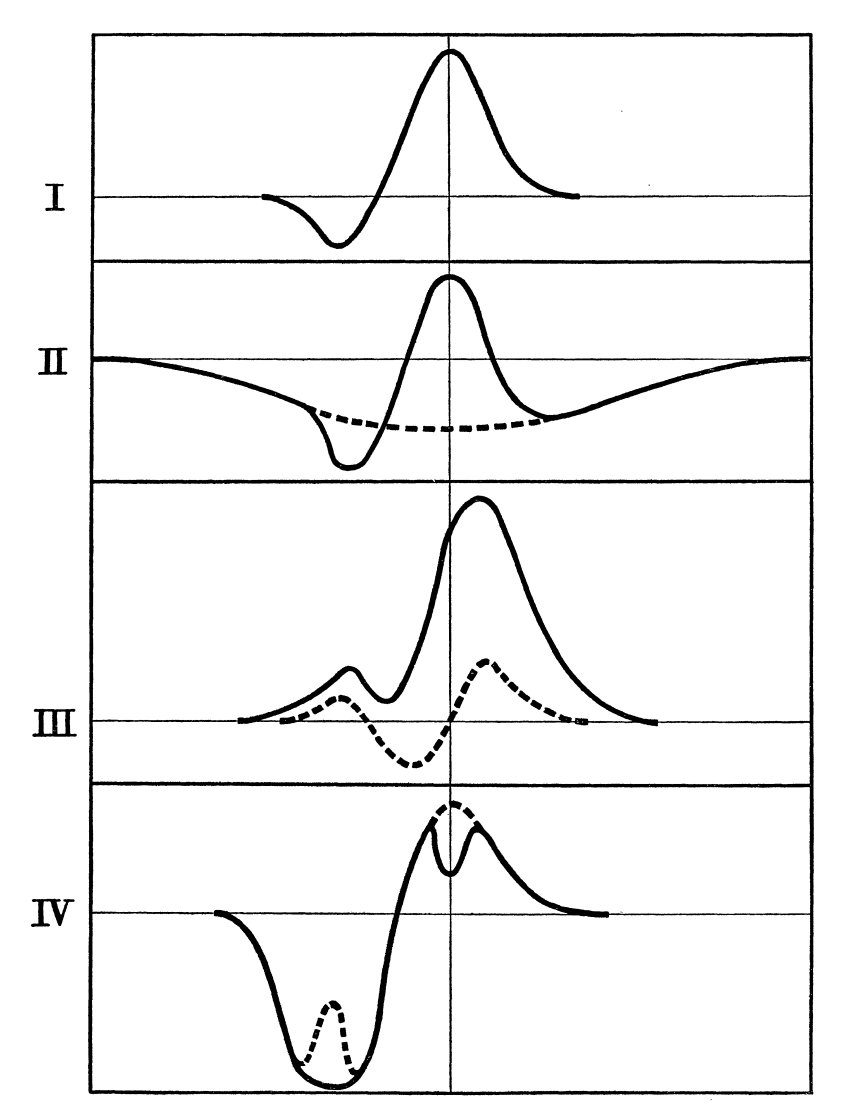
\includegraphics[scale=.30]{figures/beals class 1.png}
\caption{Primary P Cygni classes - the morphological classification of P Cygni spectra proposed by Beals (1953) \cite{1953PDAO....9....1B}.}
\end{figure}

The work also presents an early attempt at classification of P Cygni stars based on their morphologies. The classification provided by Beals is broader than modern schemes \cite{reipurth1996halpha}. In addition to the primary classes, Beals proposed a set of non-typical classes which were also considered to be P Cygni spectra. This work does not consider these non-typical classes to be P Cygni spectra but rather consider them to be a subgroup of emission line spectra. This approach is congruent with modern research \cite{vcotar2021galah}\cite{zhang2021catalog}\cite{reipurth1996halpha} which promote constraints on the classification of P Cygni and inverse P Cygni morphologies. 

Classification regimes since the 1950s have largely been manual i.e. visual inspection of spectra. However, over the last five to seven years semi-automated and automated methods have been explored by many groups. A more detailed discussion of these attempts are provided in Chapter 3.

\begin{figure}[h]
\centering
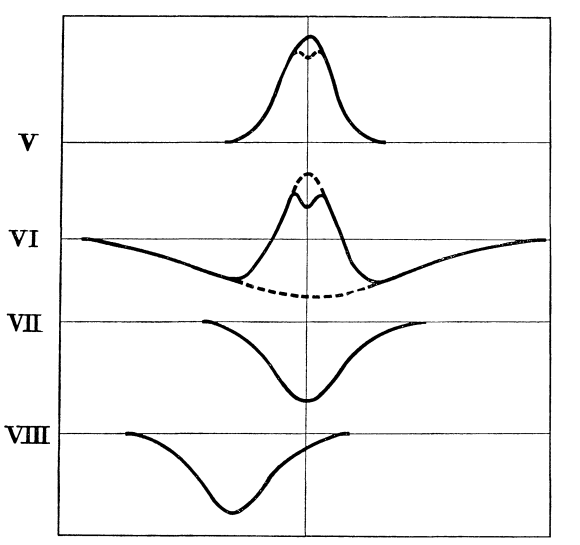
\includegraphics[scale=.50]{figures/beals class 2.png}
\caption{Non-typical P Cygni classes proposed by Beals.}
\end{figure}

\section{Importance}

The identification, classification and modelling of peculiar stars such as P Cygni and inverse P Cygni can provide significant insight into our understanding of stellar evolution and the physical processes that drive them. With the advent of modern large scale spectroscopic survey science, the importance of detecting these stars and modelling them using data driven methods has gained prominence.

Modern spectroscopic surveys generate data from millions of sources. These "million star surveys" generate a significant volume of data. Thus, it has become impractical to study these sources using manual methods. In order to generate stellar parameters from survey spectra, modern researchers rely on generalised automated pipelines. These generalised pipelines rely on templates and models that assume a non-peculiar baseline. 

It has been demonstrated that such an approach has an impact on the accurate determination of effective temperature \cite{cayrel2011halpha}\cite{amarsi2018effective}\cite{giribaldi2019accurate}. The effect on computing stellar masses has also been well documented \cite{ness2016spectroscopic}\cite{bergemann2016gaia}. Thus the identification and characterisation of peculiar stars such as P Cygni and inverse P Cygni stars has a direct impact on the accuracy of automated estimation of stellar parameters in large scale spectroscopic surveys. 

\section{The GALAH Survey}

The GALAH survey is a million star Milky Way spectroscopic survey which uses the HERMES spectrograph at the Anglo Australian Telescope \cite{de2015galah} \cite{buder2021galah+}. The GALAH survey is currently in its third data release (DR3) and contains more than 600,000 spectra. The volume of data being generated by the GALAH survey has necessitated the use of semi-automated and automated data analytics pipelines over manual methods.

\section{Goals}

REWRITE THIS

This thesis will use a novel data driven approach to cluster, classify and identify PCT stars in GALAH DR3. Once these PCT stars have been identified, the thesis will characterise these stars with reference to stellar parameters. This thesis will model the spectra using optimisation techniques and gaussian mixture models (GMM) to estimate the stellar wind velocity directly from the normalised spectra of the PCT stars (Zhang et al. 2021; Traven et al. 2015).

The focus of this literature review is twofold. One aspect of the review will be on the scientific work done on P-Cygni stars in particular and emission stars in general, and their relevance to the thesis. The second aspect will be a brief survey of recent computational methods that are relevant to the thesis, with a special focus on machine learning and signal processing methods. 





% Data
\chapter{Data}

\section{Data Acquisition}

This research project utilises the most recent open access spectral data from the GALAH survey. At the time of writing, the GALAH survey is in its third data release (GALAH DR3). GALAH DR3 comprises 678,423 spectra for 588,571 stars, of which approximately 80\% of these stars are within a radius of 2 kpc \cite{buder2021galah+}. Of the 588,571 stars, continuum normalised spectra of 588,343 have been provided.The GALAH DR3 (hereafter DR3) is accessible via the \href{https://www.galah-survey.org/}{survey website} and \href{https://datacentral.org.au/}{AAO Data Central}. DR3 provides continuum normalised spectra and errors for a majority of spectra and candidates. In the case of problematic reductions, for candidates where this is not possible, object IDs and flags have been provided. This study avoids using these problematic spectra.

The data is organised as individual \texttt{.fits} format files. Each file contains an object ID prefix (known as an "\texttt{sobject\_id}") followed the last digit in the filename which serves as the camera number suffix. Thus, the file \texttt{1705090057010093.fits} is a data file for an object with \texttt{sobject\_id=170509005701009} and contains spectral data from camera 3 (or the red camera). The blue, green and infra red cameras are denoted by the suffix 1,2 and 4 respectively.
The red camera of the HERMES spectrograph is the spectral channel with the range 6478\r{A} - 6737\r{A}\cite{sheinis2014first}. This range is of particular interest to this research as the characteristic H$\alpha$ line appears within this range. These individual files totalling 385 GB were downloaded to a Macquarie University file server and served as the data source for all research and analytical work presented in this thesis.

\begin{figure}[h]
\centering
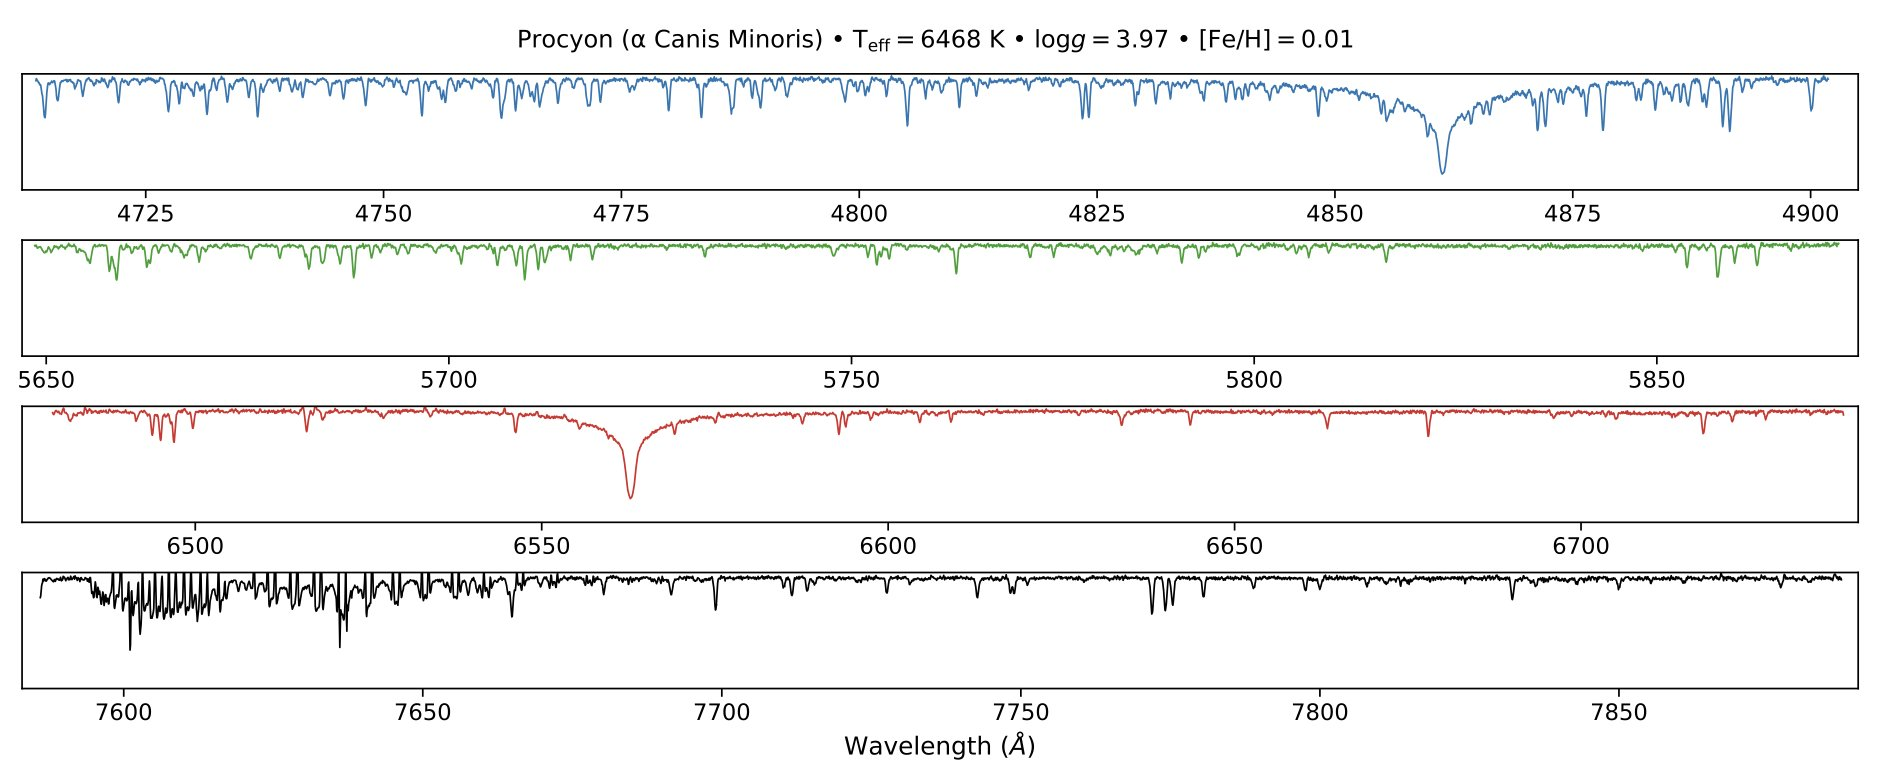
\includegraphics[scale=.25]{figures/galah cameras.jpeg}
\caption{Normalised DR3 spectral data for the star $\alpha$ Canis Minoris.}
\end{figure}

Given that spectral features are recorded across four cameras, the feature space of this data is significant. As an illustrative example, consider the red camera only. The feature space calculation is as follows.
\[\lambda_{min} = 6478\]
\[\lambda_{max} = 6737\]
\[\Delta\lambda \approx 0.06\]
Where $\Delta\lambda$ is the wavelength separation equivalent of the sampling rate of the wavelength grid of the individual spectrum. Thus the size of the wavelength grid is given by, \[N_{\lambda} = (\lambda_{max}-\lambda_{min})/\Delta\lambda \approx (6737-6478)/0.06 \approx 4317\]
This will be equal to the number of features in the red camera of a given spectrum, \[N_{f} \approx 4317\]
Thus the total number of features for the red camera across DR3 is, \[N_{T} \approx 4317\times678,423 \approx \num[round-precision=2,round-mode=figures,
     scientific-notation=true]{2928752091}\]

\begin{figure}[t]
\centering
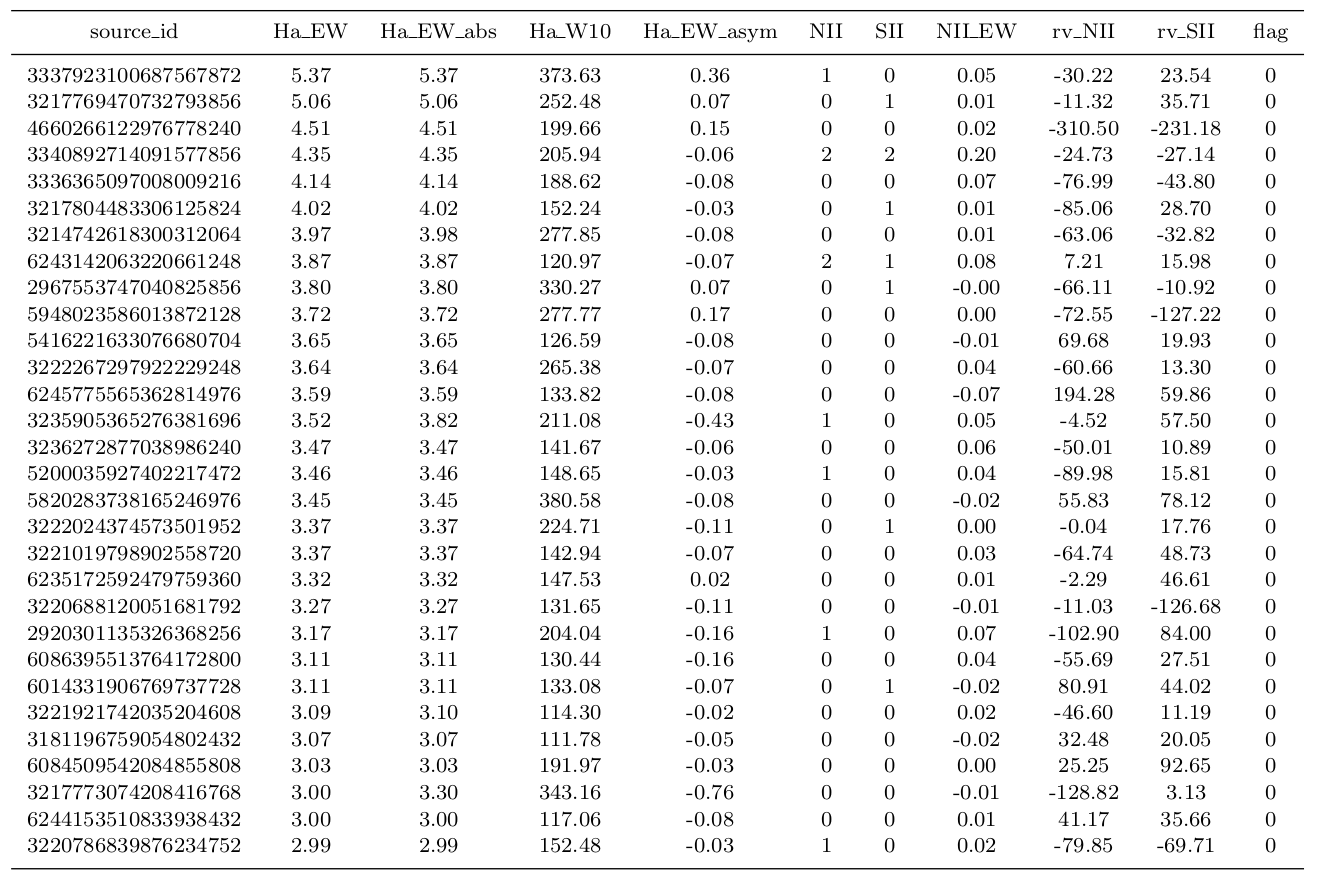
\includegraphics[scale=.35]{figures/cotartable.png}
\caption{The 30 strongest emitters. Reproduced from Čotar et al. (2021)\cite{vcotar2021galah}}
\end{figure}
This calculation naively implies the existence of a billion scale feature space, and consequently a potentially billion dimensional vector space. Thus the data analysis and machine learning strategy will have to be chosen carefully. If care is not taken during feature engineering and pre-processing steps, the volume of data will lend itself to what is colloquially referred to as the "curse of dimensionality". The curse of dimensionality implies an extraordinarily rapid growth in the difficulty of problems as the number of variables (or the dimension) increases \cite{kuo2005lifting}.

This research will also utilise a recently published dataset of H$\alpha$ candidates in DR3. Published in 2020, Čotar et al. used DR3\cite{de2015galah}, the K2-HERMES survey\cite{wittenmyer2018k2} and the TESS-HERMES survey\cite{sharma2018tess} to derive a catalogue of potential H$\alpha$ emission stars using an automated supervised machine learning pipeline. Combining data from three surveys, this study used 669,845 continuum normalised stellar spectra as a data input source and included a small fraction of repeated observations. The study identified 10,364 candidate spectra with varying degree of H$\alpha$ emission components. Summarised information of these candidates, their object IDs, including DR3 \texttt{sobject\_ids} were released via \href{https://cdsweb.u-strasbg.fr/}{CDS} as open access data. This data was presented as a single \texttt{.fits} format file. No spectral information was provided with this dataset. The 30 strongest emitters from this study are presented in Figure 2.2 above. The benefit of using this dataset over the entire DR3 is that there will be a higher chance of identifying P Cygni and inverse P Cygni spectra given essentially the pre-selection of H$\alpha$ candidates by Čotar et al. P Cygni and inverse P Cygni spectra are a subset of H$\alpha$ emission spectra. However, one limitation of using this dataset exclusively is that the potential number of identifable P Cygni stars will be limited by the number of H$\alpha$ candidates identified by Čotar et al. only. Presumably this dataset does contain all H$\alpha$ candidates in DR3 but it does not guarantee it. 

\section{Spectra as Time Series}

The normalised flux recorded by each camera as a function of wavelength can be considered to have behaviour similar to a "time series". While a monotonically increasing time axis is not included in the data, the monotonically increasing wavelength grid can serve as an analogue to the time axis. Thus a plot of normalised flux against wavelength represents the variation of a flux against wavelength similar to the variation of a time dependent quantity against the time axis.

As it shall be demonstrated in subsequent chapters, this is an unconventional yet incredibly powerful approach to spectral analysis. Precedent for this approach can be found in related fields such as chemistry and nuclear magnetic resonance (NMR) spectroscopy where NMR spectra are subjected to signal processing techniques originally developed for time series analysis \cite{nielsen2019practical}. 

\section{Data Resampling}

In order to isolate the red camera data ("camera 3"), the following process was carried out. All filenames of the DR3 \texttt{.fits} format files were read into an array. Files with the suffix "3" were then selected. Additionally the number "3" was stripped from this sub array of file names to generate a list of \texttt{sobject\_id} values. This significantly simplifies data querying and reading operations as all standard query and file read operations rely on only \texttt{sobject\_id} and not the file name that includes the \texttt{sobject\_id} and camera suffix. 

The added advantage of this approach is that it automatically excludes \texttt{sobject\_id} values for which red camera data does not exist. A list of such \texttt{sobject\_id} values is published on the GALAH survey website. However this study did not require the use of this list as the procedure above infers these \texttt{sobject\_id} values directly from the \texttt{.fits} filenames. This process results in a collection of 588,344 \texttt{sobject\_id} values. This is lower than the 588,571 total number of stars recorded by DR3. The difference is attributed to those stars for which the normalised red camera data doesn't exist. 

\begin{figure}[h]
\centering
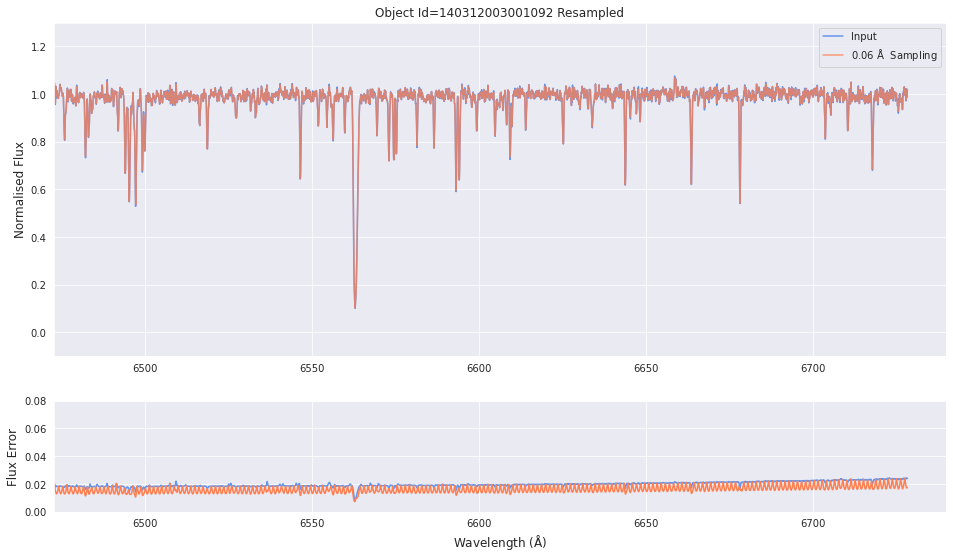
\includegraphics[scale=.40]{figures/resampling example.png}
\caption{Resampling a DR3 spectrum and it's error spectrum to a common wavelength grid.}
\end{figure}

The sampling rate for each observed spectrum can vary. For the red camera, this rate is equivalent to a wavelength separation of $\Delta\lambda$ $\approx$ 0.06 \r{A}\cite{vcotar2021galah}. The sampling rate of each spectrum from the red camera was found to vary around this value at the third decimal. For subsequent analysis each spectrum is required to be a vector of fixed size. A collection of spectra i.e. the total dataset that will be subjected to analysis must consist of a uniform set of these vectors. The advantage of this approach is that spectral features, particularly morphological features can be compared against each other more effectively. Thus the spectra under consideration were interpolated to a common wavelength grid with a sampling rate equivalent to 0.06 \r{A}. This rate was chosen so that oversampling and under-sampling would be significantly minimized. This rate is accurate to the sampling rate of each spectrum generated by the red camera to the second decimal place. 

Data resampling or interpolation in the context of spectral data is a common operation in astronomy. This work uses the \texttt{spectres} Python package \cite{carnall2017spectres} to efficiently sample all red camera spectra to the following common wavelength grid.

\[\lambda_{min} = 6472.5\]
\[\lambda_{max} = 6740\]
\[\Delta\lambda = 0.06\]

This grid was chosen based on the range of spectral values and wavelength separation observed in the raw data. Normalised spectra and their errors from the red camera were subjected to this interpolation scheme. The authors of DR3 have set the continuum value for the normalised spectra at 1. Thus, spectra for which flux values were not recorded at the tail and top end of the interpolated grid, were padded with the value 1 in order to maintain the uniformity of the common wavelength grid. Resampling is computationally intensive and thus this process was offloaded to a university science server. The resultant data and interpolated errors were saved as HDF5 files using the \texttt{.h5} file format in a single array for convenience. 

\section{Region Selection}

The total number of spectral features for the red camera is $\approx$ \num[round-precision=2,round-mode=figures, scientific-notation=true]{2928752091}. P Cygni and inverse P Cygni stars show characteristic emission and absorption profiles near the H$\alpha$ line. This observation can be exploited to significantly reduce the size of the feature space. 
The region of interest around H$\alpha$ was selected to be 6561\r{A} - 6565\r{A} \cite{traven2017galah}. Repeating the feature space calculation above it can be noted that this region is sufficiently narrow enough to reduce the feature space by a hundredfold to $\approx$ \num[round-precision=2,round-mode=figures, scientific-notation=true]{45228200} while simultaneously ensuring that it can encapsulate emission features for P Cygni and inverse P Cygni spectra. In code, this selection was implemented as a binary spectral mask which extracts the flux values for the relevant wavelength range while masking flux values outside it. A masked version of the resampled data was stored in a separate \texttt{.h5} file.



% Methods
\chapter{The Study of H$\alpha$ Emission Spectra}

\section{Context and Relevance}
P Cygni and inverse P Cygni spectra are sub classes of H$\alpha$ emission spectra \cite{zhang2021catalog}. The identification of H$\alpha$ emission spectra in large scale spectroscopic surveys is an active area of research.\cite{zhang2021catalog,vcotar2021galah,traven2015gaia}. Thus the identification of H$\alpha$ emission spectra can serve as a useful precursor to identifying P Cygni and inverse P Cygni spectra. This approach can be extremely beneficial in reducing the search space as well the feature space that may serve as input data to a detection and identification pipeline that is tuned to identify P Cygni and inverse P Cygni spectra. 

This chapter presents a brief summary of recent methods employed to identify H$\alpha$ emission spectra, in both smaller scale observations as well as large scale surveys. These are placed in the context of their importance in the identification of P Cygni and inverse P Cygni spectra.

\section{A Historical Perspective}
An atlas of high resolution line profiles with H$\alpha$ emissions was provided by Van Winckel at al. in 1993\cite{van1993atlas}. The authors provide a classification scheme for H$\alpha$ spectra based on their morphology. The spectra were identified and classified using manual methods. Direct visual inspection and measurement of the width and shape of the line profile was used to classify these spectra. In particular, wind velocity dispersions outside the primary disk of the star were used to determine the membership of candidates in each class.
A few of the classes identified by the authors include, subtype S1, narrow emission with no prominent absorption; subtype S2 which shows a clear absorption feature superimposed on a broad emission feature; and subtype S3 which shows a strong absorption feature which reaches at least the continuum level. The authors note that the radial velocities of the 59 emission lines considered were generally redshifted. It is noteworthy that this study used wind velocity dispersions to classify the spectral types. For example, S3 showed the smallest wind velocity dispersion, thus demonstrating a relationship between the morphology of the spectra and the physical processes that generate them.

\begin{figure}[h]
\centering
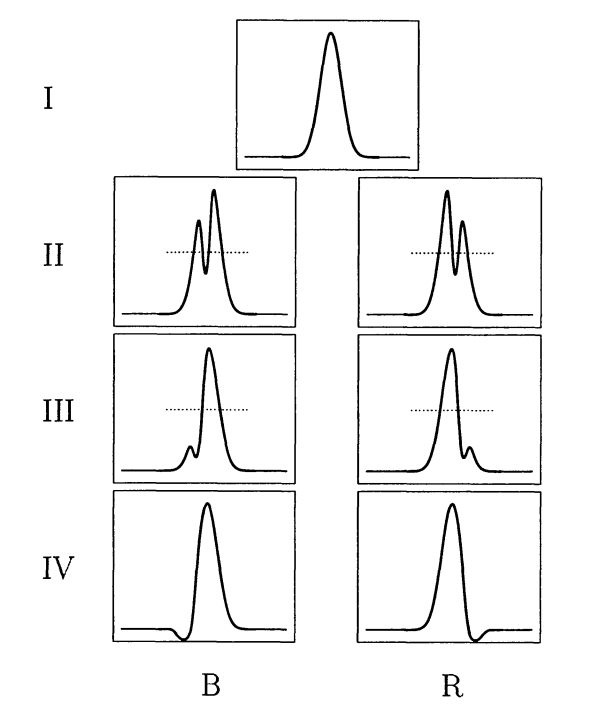
\includegraphics[scale=0.75]{figures/reipurth classes.png}
\caption{The morphology based classification scheme proposed by Reipurth et al. Depending on the location of the primary peak in relation to the secondary peak, the letters B and R are appended to the Roman numerals. They stand for blue-shifted and red-shifted respectively.}
\end{figure}

Published in 1996, Reipurth et al. studied the H$\alpha$ profiles of pre-main sequence stars using manual methods. In addition to identifying T Tauri stars and Ae/Be stars using high resolution spectra (R~50,000), the study focused on the morphological properties of P Cygni stars as well as the physical processes that generate them. The study notes the discovery of complex morphological profiles among the T Tauri, Ae/Be and P Cygni stars. 

The authors proposed a two dimensional classification scheme based on the relative height of a secondary peak compared to the primary peak, as well as whether the absorption line is blue or red shifted. The authors note the classification of 25\% symmetric profiles, 49\% blue shifted absorption profiles and 5\% P-Cygni profiles amongst the observed spectra. Of the spectra, 21\% fall into the redshifted absorption category. In addition to this morphological classification, the authors also presented wind velocities of the samples with some stars recording extremely high velocities of ~ 900km/s \cite{reipurth1996halpha}. 

The classification of P Cygni stars in this paper follow the scheme proposed by Beals in 1953\cite{1953PDAO....9....1B}. The authors have also presented a discussion comparing observed data to models in literature, particularly models that constrain mass, radii and photospheric temperatures. No specific model details for P Cygni stars were provided. Further catalogues of H$\alpha$ emission stars have been provided by Kohoutek and Wehmeyer (1997 and 1999). These catalogues contain 98 identified emission-line stars in the Northern Milky Way. These catalogues do not specifically identify P Cygni stars or inverse P Cygni stars \cite{kohoutek1999catalogue}.

The study of open clusters such as NGC 6611 and others have pushed our understanding of H$\alpha$ emission stars \cite{bonito2013spectroscopic,traven2015gaia}. Bonito et al. in particular note that for stars surrounded by active disks the morphology of the emission lines could fall into categories such as symmetric with broad wings, asymmetric and in extreme cases, P Cygni and inverse P Cygni. The authors have used the classification scheme proposed by Reipurth et al and have adhered to the type I - IV scheme with B and R suffixes to denote blue shifted and red shifted emission lines respectively. 

Traven et al. presented a catalogue of H$\alpha$ emission stars in the Gaia-ESO survey. This survey is biased towards young open clusters and consequently, the authors note a relatively large proportion of H$\alpha$ emission candidates that were identified in this work. The authors note the identification of 3765 emission stars from a sample of 22,035 spectra from the Gaia-ESO survey. This work is notable as it uses a combination of empirical rules and automated techniques like spectral fitting to sort the H$\alpha$ emission spectra into eight distinct morphological categories: single–component emission, emission blend, sharp emission peaks, double emission, P-Cygni, inverted P-Cygni, self–absorption, and emission in absorption \cite{traven2015gaia}. The Gaia-ESO survey had conducted repeat observations of about half the identified H$\alpha$ emission stars. Thus the authors were able to comment on the temporal variability of these stars. The conclusion was that while some morphological categories exhibited stability of their spectral profiles over time, P-Cygni and self-absorption profiles may not. Supplementary information of these candidates from SIMBAD, VizieR and ADS were also provided. In addition to this data, the authors have provided wind velocity estimates based on the automated curve fitting procedure. The authors note that the identification, classification and characterisation of emission stars can be valuable for automatic pipelines in large surveys (e.g. GALAH), where they can pinpoint outliers when calculating general stellar properties and abundances. Additionally, they note that the identified stars can be used in studies of star formation processes, interacting binaries and related fields of stellar physics. 

The historical review allow us to draw a number of conclusions:

\begin{enumerate}
\item These methods relied exclusively on visual inspection of spectra and manual methods to identify H$\alpha$ candidates. While this may have been a suitable approach in the past, it is extremely challenging to extend and scale these methods to datasets generated by million star all sky surveys in the modern era. Thus this project does not consider these manual methods for the detection of H$\alpha$ candidates as well as P Cygni and inverse P Cygni spectra. 

\item Morphology based classification approaches as demonstrated by Reipurth et al. and even Beals are significantly important. It was demonstrated in Chapter 1 that the variety of spectral morphologies are hypothesised to be generated due to distinct physical phenomena linked to the stellar disk and the gas that surrounds it. This research leans into this approach and relies on morphological similarities and dissimilarities as a basis for spectral classification.

\item Finally, these studies have identified P Cygni and inverse P Cygni (among other classes of spectra) as forming a subset of H$\alpha$ emission spectra. This project exploits this fact to it's logical conclusion i.e. the probability of automated detection of P Cygni and inverse P Cygni spectra can be increased if the search space and feature space of the raw data can be reduced from the complete DR3 catalog, to a much narrower subset of H$\alpha$ emission candidates identified in DR3.
\end{enumerate}

\section{Recent Developments}

The increase in data availability via large scale spectroscopic surveys has necessitated and demanded the use of semi automated and fully automated methods. Morphology based classification has been adopted by many researchers in the field and augmented by statistical methods and machine learning. In general, machine learning approaches can fall into two categories; supervised and unsupervised learning. The former relies on the availability of a suitably robust set of training examples while the latter attempts to generalise and learn from unlabelled data \cite{hastie2009elements}. A full discussion and review of machine learning methods is beyond the scope of this thesis. Techniques and methods that are relevant to this research are presented in text. Chapter 4 in particular will present a more detailed discussion on methods that are relevant to the present thesis. This section reviews four recent approaches that rely on machine learning to detect and characterise H$\alpha$ candidates, their strengths and limitations.

\subsection{K-means Clustering on APOGEE Spectra}

K-means clustering is a well known unsupervised clustering algorithm.The goal of this algorithm is to partition a set of observations into a predefined set of clusters. Each observation would belong to a cluster with the nearest mean which serves as the centroid or prototype of the cluster \cite{macqueen1967some}. Formally, given a set of $n$ observations such as \(x_1,x_2,...,x_n\) where each observation is a $d$ dimensional vector, the algorithm will partition the $n$ observations into $k$ sets $S=\{S_1,S_2,...,S_k\}$ such that within cluster variance is minimised. This objective can be represented as:

\begin{equation}
{\underset {\mathbf {S} }{\operatorname {arg\,min} }}\sum _{i=1}^{k}\sum _{\mathbf {x} \in S_{i}}\left\|\mathbf {x} -{\boldsymbol {\mu }}_{i}\right\|^{2}={\underset {\mathbf {S} }{\operatorname {arg\,min} }}\sum _{i=1}^{k}|S_{i}|\operatorname {Var} S_{i}
\end{equation}

where $\mu_i$ is the mean of the points in $S_i$. 

Using the identity:

\begin{equation}
    |S_{i}|\sum _{\mathbf {x} \in S_{i}}\left\|\mathbf {x} -{\boldsymbol {\mu }}_{i}\right\|^{2}=\sum _{\mathbf {x} \neq \mathbf {y} \in S_{i}}\left\|\mathbf {x} -\mathbf {y} \right\|^{2}
\end{equation}

It can be shown that this is equivalent to minimising the pairwise squared deviations of points belonging to the same cluster:

\begin{equation}
{\underset {\mathbf {S} }{\operatorname {arg\,min} }}\sum _{i=1}^{k}\,{\frac {1}{|S_{i}|}}\,\sum _{\mathbf {x} ,\mathbf {y} \in S_{i}}\left\|\mathbf {x} -\mathbf {y} \right\|^{2}
\end{equation}

APOGEE which is part of the Sloan Digital Sky Survey (SDSS) is a high resolution spectroscopic survey (R$\approx$ 22,500) \cite{eisenstein2001spectroscopic,blanton2017sloan}. In the absence of labelled training samples in the APOGEE survey Garcia-Dias et al. used k-means to cluster similar spectra into distinct groups \cite{garcia2018machine}. Each spectrum produced by APOGEE was treated as a $d$ dimensional vector. The number of observations $n$ was the number of spectra generated by APOGEE which was approximately 150,000. $k$ was set to 50. The authors note that they were able to separate dwarfs, sub-giants, RC and RGB stars. The authors note that the approach is sensitive to initialisation and thus sensitive to the number of clusters $k$. One major limitation of this approach is that a discrete classification in the flux space does not result in a neat organisation in the parameters' space. The other limitation being the use of manual sorting of clusters that reduced the number of clusters from 50 to 9. This implies that certain spectra were incorrectly clustered by the k-means algorithm. The authors were unable to cluster H$\alpha$ emission spectra using this method. The primary conclusion that can be drawn from this work is that k-means clustering may perform poorly if it is used to cluster and ultimately classify morphologically similar spectra such as P Cygni and inverse P Cygni. A methodology that relates the flux space, and consequently the morphology of the spectrum, to a parameter space may perform better than k-means. 

\subsection{Automated and Manual Methods on LAMOST Spectra}

The LAMOST survey is a low resolution spectroscopic survey with 10 million Milky Way stars as potential survey candidates. Zhang et al. were able to use a training and test set (labelled spectra) comprising 5,915 samples for spectral classification. This training set was based on data released by Hou et al. \cite{hou2016catalog} who developed the dataset by using a combination of emperical rules and visual examination of 10,000 LAMOST spectra. The existence of labelled data including seven P Cygni and inverse P Cygni spectra identified by Hou et al. was exploited for supervised machine learning algorithms. As such, 10 different supervised learning methods were then applied to this dataset including including KNN (K-Nearest Neighbor), RF (Random Forest), AdaBoost, Naive Bayes (MultinomialNB, GaussianNB, BernoulliNB), logistic regression, SVM (Support Vector Machine) and Artificial Neural Network (Single-hidden Layer, Three-hidden Layer) \cite{zhang2021catalog}. A comparison of the performance of these methods were not provided by the author. However they note that the k-nearest neighbour and random forest methods outperformed all other methods. A detailed discussion of these methods is omitted from this thesis as it would be beyond the scope of this project. These two supervised machine learning models were then applied to 498,588 spectra resulting in 56,574 potential H$\alpha$ emission candidates. These candidates were then visually inspected with a final candidate list of 30,048 H$\alpha$ emission spectra. A significant drawback of this approach is the reliance on manual visual inspection of spectra in building the training set as well as during classification of the identified potential H$\alpha$ emission spectra. A labelled training set with clearly identified P Cygni and inverse P Cygni spectra does not currently exist for GALAH DR3 and thus none of these methods can be extended to DR3. In the subsequent chapter, this author will demonstrate an automated method that generates such a dataset for GALAH DR3 which does not rely on manual visual inspection.

\subsection{t-SNE and DBSCAN on GALAH DR1}

As discussed previously, a stellar spectrum of vector length $d$ (a wavelength grid of size $d$), can be used to create a vector space of minimum dimensionality equal to $d$. In the case of GALAH DR1 this value is $\sim$ 4500. Conducting computational operations such as clustering and classification on a higher dimensional vector space of size $\sim$ 4500 can be problematic. In addition to the previously mentioned curse of dimensionality, researchers would also face practical limitations due to the computational intractability of working on higher dimensional vector spaces. It is often helpful to transform the data from a high-dimensional space to a low-dimensional space ensuring that meaningful properties of the original data are preserved. In the case of P Cygni and inverse P Cygni spectra, these meaningful properties would presumably include some information about the morphology of the spectrum although this may not be guaranteed. This thesis will revisit this in a subsequent chapter.

Given a total feature space (and consequently a total search space) that is made up of $n$ spectra samples of length $d$, dimensionality reduction offers an attractive approach to grapple with the curse of dimensionality and high computational complexity. Principal component analysis (PCA) is possibly the most well known dimensionality reduction technique. However, PCA may not be suitable in the context of GALAH DR1 and certainly DR3. This is explored further in subsequent chapters. More recent and novel dimensionailty reduction techniques such as t-distributed stochastic neighbour embedding (t-SNE) \cite{van2008visualizing} have been used on spectral data from GALAH DR1 \cite{traven2017galah}. Given a vector of size $d$, the application of the t-SNE algorithm will project this vector space onto a 2-dimensional vector space. The distances between data points on this 2-dimensional vector space can then be used to cluster similar data points into similar groups using a variety of popular clustering methods such as DBSCAN \cite{ester1996density} or HDBSCAN \cite{campello2013density}. A detailed discussion of this technique is presented in subsequent chapters.

\begin{figure}[h]
\centering
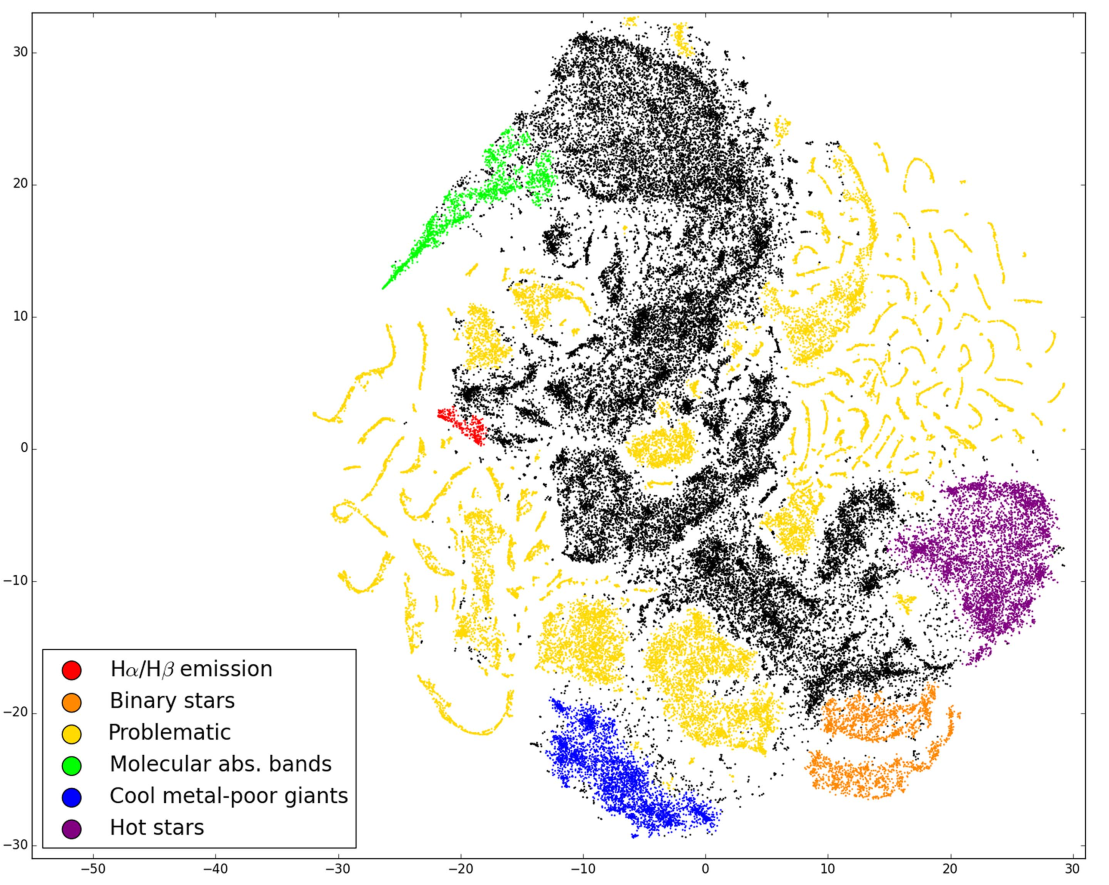
\includegraphics[scale=0.40]{figures/tsne traven.png}
\caption{The t-SNE plot with classified regions reproduced from Traven et al. \cite{traven2017galah}. The x and y axes do not have a physical meaning but serve as spanning vectors for the 2-dimensional projection space.}
\end{figure}

Using this method, Traven et al. classified six distinct stellar types and identified H$\alpha$ and H$\beta$ emission candidates in GALAH DR1. The emission candidates were further examined and 18 P Cygni spectra were identified. The identification of P Cygni spectra was a sub-component of a broader study of stellar types in GALAH DR1. The authors note that the number identified was lower than expected. The methods was not able to clearly separate P Cygni spectra from double peaked spectra, emission superimposed on absorption and other emission candidates. When examining the t-SNE plot above, it is clear that the authors were not able to distinctly separate the H$\alpha$ emission stars as a distinct cluster from the unclassified region (black). This thesis will revisit this study in subsequent chapters and demonstrate a data driven method of separating P Cygni spectra from the aforementioned categories that can overcome some of the limitations mentioned above.

\subsection{Autoencoders on GALAH DR3}

An autoencoder (AE) is a type of artificial neural network (ANN) that takes input data and reduces it to a pre-selected number of "latent features" that inhabit a low-dimensional vector space known as the latent space. The latent space can capture important features that exist in the original $d$-dimensional vectors and vector space. By processing $n$ samples of $d$-dimensional vectors, the autoencoder can then learn the latent space representation of the higher dimensional features. This is known as encoding. In the next portion of the network, the network then attempts to recover the original data from the latent vector space. The process that reduces a $d$-dimensional vector and vector space to a vector space of size $p$<$d$ is a dimensionality reduction process similar to PCA or t-SNE. The portion of the network that takes a $p$-dimensional vector from the latent space and projects it back to a $d$-dimensional vector space is essentially the inverse process of the dimensionality reduction procedure. This is known as a decoder. Since the original data is generated from the latent space, autoencoders fall into a class of ANNs called generative models (generative ANNs). Note that the latent space for an autoencoder is discrete. ANNs that can generate continuous latent spaces in this manner are known as variational autoencoders (VAEs) and are beyond the scope of this thesis. 

Autoencoders are widely used in anomaly detection applications \cite{sakurada2014anomaly}. If the autoencoder model is trained on non-anomalous data ("normal" data), the model will learn the latent space representation of non-anomalous data. If an anomalous data point is passed through the model, the autoencoder will attempt to generate this data from the latent space representation it has learned. Since the learned model was trained on non-anomalous data, the autoencoder will generate an inaccurate representation of the anomalous data. This leads to a significant prediction error between the generated anomalous data and the true anomalous data. This process can be exploited to detect time-series as well as non time-series anomalies in data.

The GALAH survey is a general all-sky survey that can be expected to generate a significantly higher proportion non-anomalous spectra. Since DR3 is not biased towards young, violent, hot stars or stellar nurseries, we expect a significantly higher proportion of spectra to show "normal" (non-anomalous) H$\alpha$ line profiles and indicate absorption. In this regime, an H$\alpha$ emission, and consequently, P Cygni and inverse P Cygni spectra are rare and anomalous. If an autoencoder is trained on normal looking spectra which do not show emission lines near H$\alpha$, it can be sensitive to H$\alpha$ emission spectra. 

\begin{figure}[h]
\centering
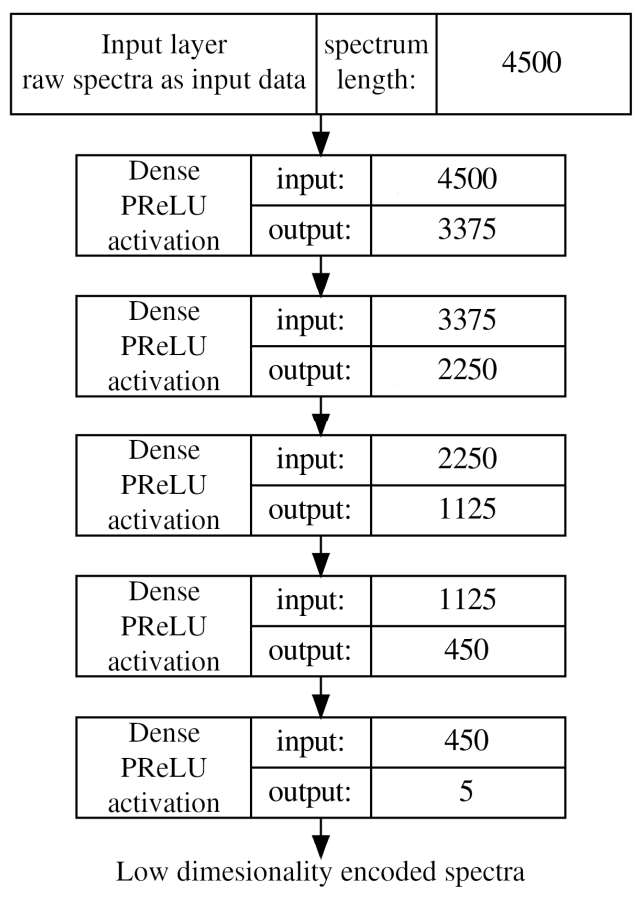
\includegraphics[scale=0.45]{figures/autoencoder.png}
\caption{An autoencoder architecture capable of detecting H$\alpha$ candidates from DR3. Reproduced from Čotar et al. \cite{vcotar2021galah}}
\end{figure}

This methodology was exploited by Čotar et al. to detect H$\alpha$ emission candidates in DR3 and other surveys \cite{vcotar2021galah}. Hyperparameter tuning is both an art and a science and requires a trial and error approach. The authors chose a network architecture that reduces a $d$-dimensional DR3 spectrum to a $p$-dimensional latent space representation. Here, $d$ = 4500 while $p$ = 5. The intervening layers and the final architecture that is capable of detecting "anomalous" H$\alpha$ emission spectra is presented below. An introduction to the H$\alpha$ candidates that were detected using this method was presented in Chapter 2. The authors did not further classify and detect P Cygni and inverse P Cygni candidates using this method. This thesis makes extensive use of this subset of DR3 data to identify and characterise P Cygni and inverse P Cygni spectra using data driven methods. This approach is discussed in detail in the next chapter. 



% Conclusion
\begin{savequote}[45mm]
If cats looked like frogs we'd realize what nasty, cruel little bastards they are. Style. That's what people remember.
\qauthor{Terry Pratchett}
\end{savequote}

\chapter{Conclusion}

Not a very interesting conclusion, however you'll need one for your thesis.




%---------------------------------------------------------- 
% APPENDICES
% include chapters as needed (will be numbered differently)
%---------------------------------------------------------- 
\appendix

\chapter{Appendix}

\section{Appendix C - Chapter 6}

\begin{table}[!htb]
\begin{center}
\begin{tabular}{|l|l|}
\hline
\textbf{count} & 7067.000000 \\ \hline
\textbf{mean} & 0.532952 \\ \hline
\textbf{std} & 0.444046 \\ \hline
\textbf{min} & 0.220042 \\ \hline
\textbf{25\%} & 0.280778 \\ \hline
\textbf{50\%} & 0.388232 \\ \hline
\textbf{75\%} & 0.562633 \\ \hline
\textbf{max} & 5.055410 \\ \hline
\end{tabular}
\caption{EW distribution summary statistics for emission-line stars identified in GALAH DR3}
\label{table:draglift1}
\end{center}
\end{table}

\begin{table}[!htb]
\begin{center}
\begin{tabular}{|l|l|}
\hline
\textbf{count} & 10364.000000 \\ \hline
\textbf{mean} & 0.539950 \\ \hline
\textbf{std} & 0.420590 \\ \hline
\textbf{min} & 0.250070 \\ \hline
\textbf{25\%} & 0.298572 \\ \hline
\textbf{50\%} & 0.392470 \\ \hline
\textbf{75\%} & 0.592625 \\ \hline
\textbf{max} & 5.369496 \\ \hline
\end{tabular}
\caption{EW distribution summary statistics for emission-line stars identified by Čotar et al. (various surveys).}
\label{table:draglift1}
\end{center}
\end{table}

\begin{figure}[!htb]
\centering
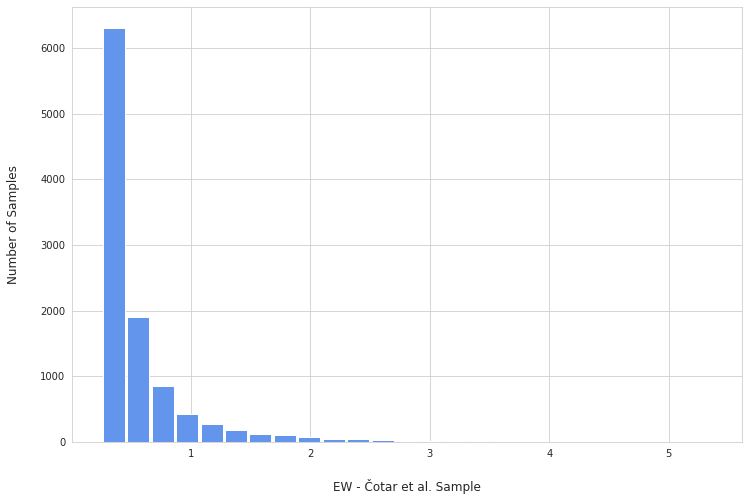
\includegraphics[scale=0.50]{figures/EW hist cotar.png}
\caption{The equivalent width (EW) distribution of the inverted difference spectra of the emission-line spectra provided by Čotar et al. Here EW > 0.25. Note that this sample contains additional spectra not in GALAH DR3.}
\end{figure}






%---------------------------------------------------------- 
% BACK
% list of symbols / references / index etc
%---------------------------------------------------------- 
\backmatter

% your thesis may not need this, so comment out or delete the following line
\chapter{List of Symbols}

% please change this list to suit your thesis

The following list is neither exhaustive nor exclusive, but may be helpful.
\begin{list}{}{%
\setlength{\labelwidth}{24mm}
\setlength{\leftmargin}{35mm}}
\item[$a$, $b$, $c$, $d$\dotfill] annihilation operators
\item[$a^\dagger$, $b^\dagger$, $c^\dagger$, $d^\dagger$\dotfill] creation
operators
\end{list}


% Bibliography, in BibTeX format (the references.bib file)

\bibliography{references}

\end{document}
